%------------------------------------------------------------------------------
%  DOCUMENT CONFIGURATION
%------------------------------------------------------------------------------

\documentclass[twoside, a4paper, titlepage]{article}

%------------------------------------------------------------------------------
%  PACKAGES
%------------------------------------------------------------------------------

\usepackage[utf8]{inputenc}
\usepackage[english]{babel}
\usepackage{csquotes} % Recommended

\usepackage[
  backend=biber,
  style=authoryear-ibid,
  maxcitenames=3,
  maxbibnames=100
]{biblatex}
\addbibresource{sources.bib}

\usepackage{fancyhdr} % Required for custom headers
\usepackage{lastpage} % Required to determine the last page for the footer
\usepackage{extramarks} % Required for headers and footers
\usepackage{graphicx} % Required to insert images
\usepackage{rotating} % Required for sideways figure
\usepackage{parskip} % Required for paragraph styling
\usepackage{float} % For having figures inline
\usepackage{amsmath}
\usepackage{amssymb}
\usepackage{hyperref} % For links
\usepackage{blindtext}
\usepackage{outlines}
\usepackage{tabularx}
\usepackage{minted}

\usepackage{tikz}
\restylefloat{figure}

%------------------------------------------------------------------------------

% Margins
\topmargin=-0.45in
\evensidemargin=0in
\oddsidemargin=0in
\textwidth=6.5in
\textheight=9.0in
\headsep=0.25in

% Numbering
% \setcounter{secnumdepth}{-1}

% Sans Serif Font
\renewcommand\rmdefault{cmss}

% Line spacing
\linespread{1.1}

% Images
\setlength\fboxsep{0pt}
\setlength\fboxrule{0.5pt}

\setlength\parskip{1.2em} % Space between paragraphs
\setlength\parindent{0pt} % Removes all indentation from paragraphs

% Tikz
\def\checkmark{ \tikz\fill[scale=0.4](0,.35) -- (.25,0) -- (1,.7) -- (.25,.15) -- cycle; }

%------------------------------------------------------------------------------
% TITLE PAGE
%------------------------------------------------------------------------------

\begin{document}

% Definition of blocks:
\tikzset{%
  block/.style    = {draw, thick, rectangle, minimum height = 3em,
    minimum width = 3em},
  sum/.style      = {draw, circle, node distance = 2cm}, % Adder
  input/.style    = {coordinate}, % Input
  output/.style   = {coordinate} % Output
}

\pagestyle{empty}

\newcommand{\reporttitle}{Blockchain-mediated Layered Access to Data}
\newcommand{\reportauthor}{Frederick Lindsey}
\newcommand{\reportsupervisor}{Dr. William Knottenbelt}
\newcommand{\reporttype}{BEng. Individual Project Report}

\begin{titlepage}

\newcommand{\HRule}{\rule{\linewidth}{0.5mm}}

\centering % Center remainder of the page
\vspace{1cm}


%-------------------------
%	HEADING SECTIONS
%-------------------------

\textsc{\LARGE \reporttype}\\[1.5cm]
\textsc{\Large Imperial College London}\\[0.5cm]
\textsc{\large Department of Computing}\\[0.5cm]

%--------------------------
%	TITLE SECTION
%--------------------------

\includegraphics[width = 4cm]{images/imperial_college_london_coat_of_arms}\\[0.5cm]

\HRule \\[0.4cm]
{ \huge \bfseries \reporttitle}\\
\HRule \\[1.5cm]

%--------------------------
%	AUTHOR SECTION
%--------------------------

\large
\begin{minipage}{0.5\textwidth}

\textit{Author:}\\
\reportauthor

\end{minipage}%
\begin{minipage}{0.5\textwidth}

\textit{Supervisor:}\\
\reportsupervisor

\end{minipage}

\vspace{7cm}
\makeatletter
\@date

\makeatother
\end{titlepage}


%------------------------------------------------------------------------------
% CONTENT
%------------------------------------------------------------------------------

% MOTIVATION
% CONTRIBUTIONS
% RESULTS

% APPLICABILITY
\abstract

\thispagestyle{plain}
\pagenumbering{roman}
\setcounter{page}{1}

Over the last several hundred years, the way we access and manage the world's data has radically changed. Recounting medieval times when there was little to no public record of a person's assets or information, this presents a stark comparison to today's society, where our data and identities are traded on a global market, often without our knowledge. This thesis, and it's accompanying proof of concept, seeks to describe a method of reinstating the ownership of data that was once commonplace in previous centuries, without compromising on the free flowing and global nature of communication today.

% TODO: Add information from report findings
TODO: Add information from report findings and more focused text

% Discuss motivation briefly

% Objective of determining whether a decentralised system can be successful

% Whilst possible, not ready in the slightest


% Acknowledge those who've technically or otherwise helped with completing the project
\renewcommand{\abstractname}{Acknowledgements}
\abstract

\thispagestyle{plain}
\pagenumbering{roman}
\setcounter{page}{2}

\begin{center}
  I'd like to thank Professor William Knottenbelt and Dr. Robert Learney for their support and guidance through this project. Their support was instrumental in this project and greatly appreciated.

  I'd also like to thank Professor Chris Hankin and Dr. Melek Somai for their involvement.
\end{center}


% Set up the header and footer
\pagestyle{fancy}
\pagenumbering{arabic}
% \lhead{\docAuthorName} % Top left header
\rhead{\firstxmark} % Top right header
\lfoot{\lastxmark} % Bottom left footer
\cfoot{} % Bottom center footer
\rfoot{Page\ \thepage\ of\ \pageref{LastPage}} % Bottom right footer
\renewcommand\headrulewidth{0.4pt} % Size of the header rule
\renewcommand\footrulewidth{0.4pt} % Size of the footer rule

%------------------------------------------------------------------------------
% TABLE OF CONTENTS
%------------------------------------------------------------------------------

\setcounter{tocdepth}{3}

\tableofcontents

%------------------------------------------------------------------------------
% INTRODUCTION AND PREFACE
%------------------------------------------------------------------------------

% MOTIVATION
% OBJECTIVES
% CONTRIBUTIONS
\section{Introduction}

% - Privatisation of data
%   - Google, Facebook, NHS, Banks, retail stores (loyalty programs)
%   - Data Protection Act (limitations and corporate-focus)
% - User choice (who do I want to have my data and how)
% - Online identities
%   - Global identity tracking
%   - Conglomerate identity providers
\subsection{Motivation}

Over the last 350 years, the general public has, often unwittingly, handed their right to privacy over to corporations, conglomerates, and governments. This has occurred through the exchange of personal data for the convenience of the modern world. Some might argue, however, that these transactions have not occurred in good faith and been equally beneficial to both parties.
\newline
The origin of such transactions in the UK might be attributed to the introduction of paper money in 1694 by the Bank of England~\cite{bankofengland:2016:online}. The introduction of paper currency gave an opportunity to the Bank of England to start collecting data on the exchange of money nationally. At the time it is unlikely that any person exchanging gold for paper currency was aware of the impending social shift, likely more concerned with the convenience afforded to them. Before this time, a person might have kept their savings 'under the mattress' and almost certainly would not have shared information relating to their wealth with another party. Whilst bank notes were introduced as a means to raise funds for war, the seed for a data revolution was inadvertently sewn. Whilst no unique identities were shared at this point, they would be in years to come.

Fast forward several hundred years and we find ourselves in a society where it is commonplace to rely on few key corporations and organisations to control information nationally and internationally. As (probably) the world's most popular social network~\cite{worldmapsocialnetworks:2017:online} it is clear from Facebook's terms and conditions~\cite{facebookterms:2015:online} that our use of the social network is subject to a few key conditions which restrict and change the status quo of our privacy as users. Foremost, it is apparent that whilst content posted on Facebook remains the property of the owner, Facebook has the right to use it how it wishes (as per the IP license) and hence is the controller of that data. One might choose to post it on Facebook, but one cannot stop Facebook using their content without removing it from all of Facebook's services and ensuring everyone with whom one has shared it with has also removed it from Facebook. Furthermore this allows Facebook to use any content posted for machine learning, training systems and providing commercial services using the intelligence gained from the distribution of content on the Facebook network. As someone who cares for their privacy, it is my opinion that this is not an acceptable status quo.

Notably, Facebook is not the only social network with this perspective on user privacy. Twitter also shares a very similar stance~\cite{twittertos:2017:online} and it is generally observed with most similar companies.

\begin{displayquote}{
  "\textbf{When it comes to control over our own data, health data must be where we draw the line.}"~\cite{wilbankstopol:2016:article}
}\end{displayquote}

% TODO: Swiss health identity card data

% - Privatisation of data
%   - Google, Facebook, NHS, Banks, retail stores (loyalty programs)
%   - Data Protection Act (limitations and corporate-focus)
% - User choice (who do I want to have my data and how)
% - Online identities
%   - Global identity tracking
%   - Conglomerate identity providers


At the core of the motivation for this project lay several issues corresponding to the way in which society has been manipulated over time. It is my belief that we find ourselves in the current position without any ownership of our data because we've been keen (even greedy) as a society to reap the benefits of our data without considering the longer term security effects. We have neglected our responsibility to care for our data.

Below, I have highlighted the key domains in which we lack control that we should have over our personal data. Whilst written as a piece of fiction, we should be aware and concerned that ignoring the social issues with data transfer allows a world to form much similar to that of George Orwell's 1984~\cite{orwell:1984:book} - we consider the likes of corporations synonymous with that of the 'Big Brother' character.

\subsubsection{Commoditisation of personal (and private) data}

There is no doubt that search tools such as those offered by Google and Microsoft, retail stores such as those offered by Amazon, and social networks such as Facebook and Twitter, dramatically enhance our lives and give us capabilities we would never have otherwise. Often as consumers we are eager to accept these benefits without considering the means by which they are offered to us.

% TODO: Freedom to use personal data
% \subsubsection{Freedom to use personal data}


\subsection{Objectives}

This project aims to re-imagine how we share data by prioritising the privacy, control, and availability of personal data. It is my belief that through decentralisation it is possible to have a system which no one entity controls or owns, but which every willing and able entity can participate in, privately. In the context of this project, privacy concerns the underlying data, not the transparency of data transactions occurring.

The primary objective of this project is to \textbf{discover whether a fully decentralised, private data sharing platform can exist}. The meaning of private in this context refers to hiding the content of the underlying data. The following secondary objectives follow from the primary objective:

\begin{itemize}
  \item \textbf{End-to-end Encryption} \\
  Must only share data which is encrypted and decrypted client-side. No unencrypted data flow of content is allowed.
  \item \textbf{Decentralisation} \\
  Wherever possible a decentralised service should be favoured over a centralised one.
  \item \textbf{Real-world Use} \\
  Establish whether a system would be practical for use by real people under real circumstances with real data. A practical application is central to the project's success.
  \item \textbf{Permissions} \\
  A user should be able to administer permissions for data they own
  \item \textbf{Group access} \\
  A successful implementation will allow group access under the same permissions as are available to an individual
  \item \textbf{Accessibility} \\
  The project should use technologies that can be integrated and used by current software where applicable.
\end{itemize}


\subsection{Contributions}



%------------------------------------------------------------------------------
% BACKGROUND
%------------------------------------------------------------------------------

\section{Background}

\subsection{Distributed Ledger Technology}

\subsubsection{Introduction to Distributed Ledger Technology}

Distributed ledger technology (DLT) is a recent invention which endeavours to make data publicly accessible through a decentralised system, providing no single point of failure. A DLT provides transparency where traditional centralised systems fall short and allows any willing and able party to be a part of the decentralised network. Furthermore, a DLT provides no easy way for any network moderator or specific party to control or override the network without the consensus of a significant number of the network's members. Combined, this technology introduces an entirely new way of dealing with transactional data and, as implemented below, any sort of data having a lifecycle.

\subsubsection{Blockchain}

The Blockchain~\footnote{\href{https://www.blockchain.com/}{Blockchain (https://www.blockchain.com)}} is the underlying technology that is used by cryptocurrencies such as Bitcoin~\footnote{\href{https://bitcoin.org/en/}{Bitcoin (https://bitcoin.org)}}. Since Blockchain was the first widely-available distributed ledger technology, most distributed ledger technologies since have chosen to adopt the blockchain name to refer to this architecture.

A traditional database is implemented such that it only maintains one current state for a given dataset~\footnote{Some databases have features allowing the user to view state (not transactions) over time (e.g. \href{https://www.postgresql.org/docs/6.3/static/c0503.htm}{PostgreSQL's Time Travel}) but these are not common and often deprecated} rather than transactions. In contrast, a blockchain, as the name would suggest, maintains a 'chain' of blocks of transactions that are agreed by the network forming a history of the chain's life. These blocks are formed of groups of transactions and are totally ordered across nodes in the network. It follows therefore that every node needs to have the entire history of the network, and that the provenance and origin of any given commodity, the unit of measure of a transaction, is maintained.

Whilst the above summarises the differences in the way a blockchain holds data compared to a traditional database, the differences in transaction ordering are far more fundamental and interesting. Consensus is used across a blockchain network to establish the most popular chain of transactions. It is possible for many chain possibilities to exist at any given time, but the longest chain is always assumed to be the main chain. Once a client has accepted a transaction (as part of a block), and it therefore forms part of their chain, it is not possible to choose another chain where this transaction has not been accepted (as part of the same block).

\subsubsection{Blockchain Consensus}

A few of the most popular methods of achieving consensus in a blockchain, and therefore total ordering, are listed below.

\begin{itemize}
  \item
    \textbf{Proof Of Work (PoW)}
    \textit{The majority of compute power in the network is held by honest members.~\footnote{Used by Bitcoin and Ethereum (pre-Serenity). \href{https://en.bitcoin.it/wiki/Proof_of_work}{Bitcoin Wiki}}}
  \item
    \textbf{Proof Of Stake (PoS)}
    \textit{The majority of stake (currency) in the network is held by honest members.~\footnote{Planned to be used by Ethereum (Serenity release and beyond). \href{https://www.cryptocompare.com/coins/guides/the-ethereum-releases-of-frontier-homestead-metropolis-and-serenity/}{Crypto Compare}}}
  % \item
  %   \paragraph{Byzantine Agreement (BA)}
  % \item
  %   \paragraph{Tendermint (TM)}
  % \item
  %   \paragraph{Stellar Consensus Protocol (SCP)}
\end{itemize}

\paragraph{Proof of Work}

Originally proposed as a method for countering denial of service attacks, Hashcash, authored by \cite{hashcash:1997:misc} and re-evaluated in \cite{hashcash:2002:online}, is the original proof of work scheme. The idea is that using cost-functions~\footnote{A cost-function should be parametrically expensive to compute, but efficiently verifiable. \cite{hashcash:2002:online}}, the hash of some $x$ is computed such that the left-most $n$ bits are equal to $0$. Since the hash of any two similar values is very different, as shown in program code \ref{code:example_keccak_unpredictability}, a cost-function designed in this way is difficult to compute.

\begin{listing}[H]
  \centering
  \begin{minted}{bash}
> hash('keccak256').update('Hello World!0').digest().toString('hex')
'2c6e6992915d52790a3625b459a0e7a1540a7770a6582f926d0119266b6f9f51'
> hash('keccak256').update('Hello World!1').digest().toString('hex')
'4d880de6488218d7153abeacff100608191ea63cccdd9894a602e8b3c959a276'
> hash('keccak256').update('Hello World!3').digest().toString('hex')
'f016006873889f59798ff191de74c0953892b38f77dbefc67b45af5ac705fcff'
  \end{minted}
  \caption{
    Variance between hashes of similar values
  }{
    Three similar values, shown to have very different hashes using the Keccak 256-bit hash function.
  }
  \label{code:example_keccak_unpredictability}
\end{listing}


As stated in the original Bitcoin paper (\cite{bitcoin:2008:misc}), the cryptocurrency uses Hashcash to provide block validation and to chain blocks of transactions together. As per Hashcash, the hash of the next (proposed) block must have the top $n$ bits set to zero. This value is how the network self-manages, adjusting $n$ according to a moving average of the number of blocks per hour. The hash of any particular block is computed by hashing the previous block's hash, the content of the block, and some nonce (a random value). As the nonce is incremented the hash of the block varies hugely and with sufficient iterations, the block will match the requirements of the next block.

Given the nonce we have a function difficult to compute but easy to verify, providing integrity to the underlying transactions, and ensuring that should any block be changed that's been verified, all child blocks (recursively) must be recomputed. If we assume that $51+\%$ of the compute power in the network is on honest nodes, then the longest chain will also be honest. Any malicious party would need to outpace the honest nodes in the network in order to take control and re-write the chain. The so-called $51\%$ attack is the most significant security threat to the proof-of-work model.

The proof-of-work model summarised above is used in the Bitcoin and Ethereum cryptocurrency systems for their main networks as of 15th June 2017.

\paragraph{Proof of Stake}

Intended as an alternative consensus mechanism to Proof of Work (PoW), Proof of Stake (PoS) uses a party's stake in the network to determine it's voting rights to the new block. This is in direct constrast to PoW which uses a party's compute power.

Neither Ethereum nor Bitcoin currently use proof of stake, although Ethereum is intending to use it in future releases. It remains a controversial consensus method, and as such is only summarised here.

As described by Ethereum~\footnote{\href{https://github.com/ethereum/wiki/wiki}{\textit{Ethereum Wiki}}}, there are two major consensus algorithms within the PoS category, \textbf{chain-based} and \textbf{Byzantine Fault Tolerance (BFT-style)}.

Within both of the major algorithms is the concept of a validator. A validator is someone who locks their ether as a deposit for a period of time. During this time, they are a current validator. In order to propose a block a party must be a current validator.

A chain-based algorithm uses a pseudo-random selection picking a current validator who is able to propose a block for a short time period. After this time period the validator changes. As in PoW the block proposed must point to some previously mined block, assuring a continuous chain is formed.

The BFT-style algorithm extends the idea behind the chain-based algorithm but over multiple rounds. In each round random validators are chosen to propose blocks. Over the rounds a consensus on a canonical block is reached, extending the chain.

% \paragraph{Byzantine}

% \paragraph{Stellar Consensus Protocol}

% \paragraph{Tendermint}

\subsubsection{Ethereum}

Ethereum extends the blockchain's uses beyond the direct exchange of currency and into the world whereby autonomous and publicly verifiable organisations and parties can live on the blockchain. By allowing the creation of so-called 'smart contracts', entities are established as part of the blockchain which can receive transactions from external parties (you and I). Through these transactions, the state of the contract is updated allowing the contract to function as a state transition system. Documentation and a Wiki page are the main sources of information on the Ethereum ecosystem~\footnote{\href{http://ethdocs.org/en/latest}{\textit{Read the Docs}, http://ethdocs.org/en/latest}}.

\paragraph{Ethereum Virtual Machine}

In the original blockchain, underpinning Bitcoin, a portion of every transaction is taken up by the script associated with performing it. In essence, this script represents the contract of the transaction. With Ethereum, the script transmitted with a transaction should be compatible with the Ethereum virtual machine (EVM). The EVM houses an environment where any conceivable computation of arbitrarily complexity can be achieved (turing-complete), with instructions authored and compiled in languages similar to JavaScript~\footnote{\href{https://solidity.readthedocs.io/en/develop/}{\textit{Solidity (Read the Docs)}, https://solidity.readthedocs.io/en/develop/}} and Python~\footnote{\href{https://github.com/ethereum/wiki/wiki/Serpent}{\textit{Serpent Wiki}, https://github.com/ethereum/wiki/wiki/Serpent}}. Through these languages contract code is compiled and 'activated' on an Ethereum network where it will be interacted with by externally-owned accounts (EOA). These interactions allow the realisation of the utility provided by the Ethereum network; the cryptographically secure underpinnings and distributed compute.

\paragraph{Decentralised Applications (ÐApps)}

With the EVM summarised above, we move to understanding the architecture of applications hosted by the Ethereum network and run on the EVM. A decentralised application (ÐApp) is an application whose's logic is hosted on the Ethereum network (through the medium of smart contracts) and interacting with the logic is done through a decentralised interface.

\subsubsection{Merkle Trees}

The importance of Merkle trees in the architecture and implementation of decentralised systems cannot be underestimated. When discussing the hashing of blocks above, the hash at the core of the block is that representing the integrity value of the transactions the block contains. As will be evidenced in the discussion of decentralised storage platforms, Merkle trees are at the very core of hashing the transactions in a block.

\cite{merkle:1988:inbook} authored a scheme to build trees where the content of a node could be validated as a function of the hash of other nodes. First one chooses a suitable hash function, and applies this to all leaf nodes in a possible tree. Then, one must apply the same hash function applied to the leaf nodes to the parent nodes such that every parent's hash is the hash of the sum of it's own value and the hashes of it's direct children. This structure results in a tree as in figure \ref{fig:example_merkle_tree}.

\begin{figure}[H]
  \centering
  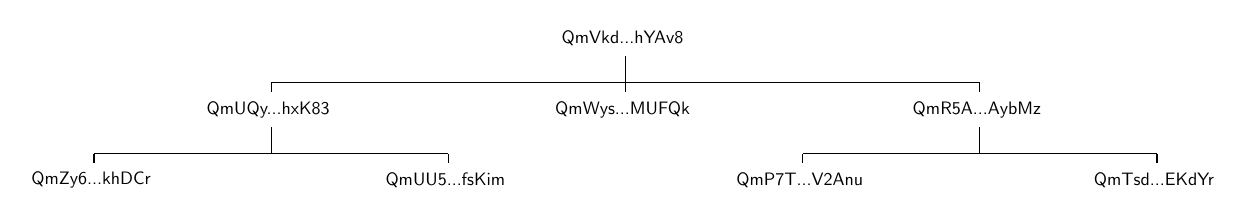
\begin{tikzpicture}[scale = 0.45, every node/.style={scale = 0.65}, every node/.append style={fill = white, rounded corners = 2pt, inner sep = 2pt, align = center}]

  \node at (0, 0) { QmVkd...hYAv8 };

  \draw (0, -0.5) -- (0, -1.5);
  \draw (-10, -1.25) -- (10, -1.25);
  \draw (-10, -1.25) -- (-10, -1.5);
  \draw (10, -1.25) -- (10, -1.5);

  \node at (-10, -2) { QmUQy...hxK83 };
  \node at (0, -2) { QmWys...MUFQk };
  \node at (10, -2) { QmR5A...AybMz };

  \draw (-10, -2.5) -- (-10, -3.25);
  \draw (-15, -3.25) -- (-5, -3.25);
  \draw (-15, -3.25) -- (-15, -3.5);
  \draw (-5, -3.25) -- (-5, -3.5);

  \draw (10, -2.5) -- (10, -3.25);
  \draw (15, -3.25) -- (5, -3.25);
  \draw (15, -3.25) -- (15, -3.5);
  \draw (5, -3.25) -- (5, -3.5);

  \node at (-15, -4) { QmZy6...khDCr };
  \node at (-5, -4) { QmUU5...fsKim };

  \node at (5, -4) { QmP7T...V2Anu };
  \node at (15, -4) { QmTsd...EKdYr };

  \end{tikzpicture}
  \caption{
    Example merkle tree
  }
  \label{fig:example_merkle_tree}
\end{figure}



\subsection{Proxy Re-Encryption}

\subsubsection{Introduction to Proxy Re-Encryption}

\begin{displayquote}{
  \textbf{"In a proxy re-encryption scheme a semi-trusted proxy converts a ciphertext for Alice into a ciphertext for Bob without seeing the underlying plaintext"}~\cite{greenateniese:2006:article}
}\end{displayquote}

Introduced as 'atomic proxy cryptography'~\cite{bbs:1998:book}, proxy re-encryption is the process of taking a message $M_a$, encrypted for a party $P_a$, and re-encrypting it such that it is readable by party $P_b$. Through the re-encryption process, the message is never decrypted by the proxy, such that the data is never revealed to any parties (including the proxy) other than the delegator and delegatees. This process relies on the functional relationship between the two ciphertexts, with the characteristics of the proxy re-encryption processed determined by the topology of this function.

\begin{figure}[H]
  \centering
  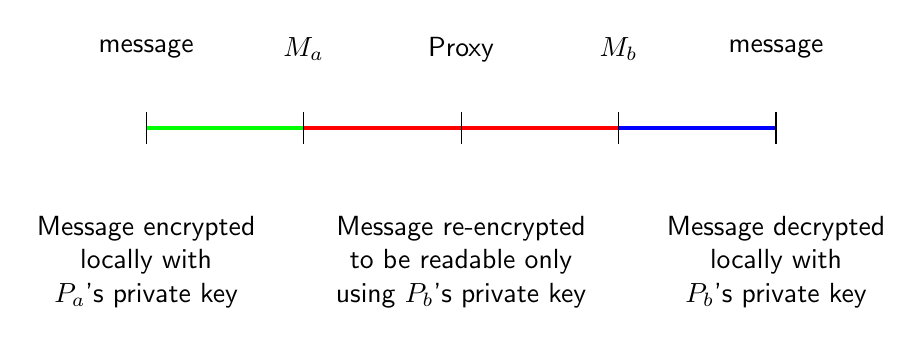
\begin{tikzpicture}

  \node at (0, 1)   {message} ;
  \node at (2, 1)   {$M_a$}   ;
  \node at (4, 1)   {Proxy}   ;
  \node at (6, 1)   {$M_b$}   ;
  \node at (8, 1)   {message} ;

  \draw [very thick, green] (0,0)   -- (2,0)   ;
  \draw [very thick, red]   (2,0)   -- (6,0)   ;
  \draw [very thick, blue]  (6,0)   -- (8,0)   ;
  \draw                     (0,-.2) -- (0, .2) ;
  \draw                     (2,-.2) -- (2, .2) ;
  \draw                     (4,-.2) -- (4, .2) ;
  \draw                     (6,-.2) -- (6, .2) ;
  \draw                     (8,-.2) -- (8, .2) ;

  \node[align=center, below] at (0, -1)%
    {Message encrypted\\locally with\\$P_a$'s private key};
  \node[align=center, below] at (4, -1)%
    {Message re-encrypted\\to be readable only\\using $P_b$'s private key};
  \node[align=center, below] at (8, -1)%
    {Message decrypted\\locally with\\$P_b$'s private key};

  \end{tikzpicture}
  \caption{
    Journey of a message using a proxy re-encryption scheme.
  }
\end{figure}


In figure \ref{fig:pre_example}, whether data is handled or manipulated by a fully trusted entity (a delegator or delegatee) or not is indicated using green/blue and red lines respectively.

The encrypted message $M_a$ is passed to the semi-trusted proxy along with the re-encryption key ( some $f(SK_a, PK_b)$\footnote{$SK_x$ represents the secret (private) key of a party $x$, $PK_x$ represents the public key of a party $x$.})

Below I discuss the contributions of various authors through the history of proxy re-encryption and the available schemes that might be suitable for a project focused on providing secure data sharing and storage.

% Delegation – allows a message recipient (keyholder) to generate a re-encryption key based on his secret key and the key of the delegated user. This re-encryption key is used by the proxy as input to the re-encryption function, which is executed by the proxy to translate ciphertexts to the delegated user's key. Asymmetric proxy re-encryption schemes come in bi-directional and uni-directional varieties.

% - In a bi-directional scheme, the re-encryption scheme is reversible—that is, the re-encryption key can be used to translate messages from Bob to Charlie, as well as from Charlie to Bob. This can have various security consequences, depending on the application. One notable characteristic of bi-directional schemes is that both the delegator and delegated party (e.g., Charlie and Bob) must combine their secret keys to produce the re-encryption key.
% - A uni-directional scheme is effectively one-way; messages can be re-encrypted from Bob to Charlie, but not the reverse. Uni-directional schemes can be constructed such that the delegated party need not reveal its secret key. For example, Bob could delegate to Charlie by combining his secret key with Charlie's public key.

% Transitivity – Transitive proxy re-encryption schemes allow for a ciphertext to be re-encrypted an unlimited number of times. For example, a ciphertext might be re-encrypted from Bob to Charlie, and then again from Charlie to David and so on. Non-transitive schemes allow for only one (or a limited number) of re-encryptions on a given ciphertext. Currently, there is no known uni-directional, transitive proxy re-encryption scheme. It is an open problem as to whether such constructions are possible.

\subsubsection{Atomic Proxy Cryptography}

Recognising that it is intuitive to expect any good cryptography scheme to disallow any untrusted party to re-encrypt a ciphertext, \cite{bbs:1998:book} suggests that perhaps it is desirable to allow re-encryption of a ciphertext, but only for specific delegatees. This is subject to doing so atomically, i.e. without revealing the underlying ciphertext, and without knowledge of the delegator or delegatee being exposed in the process. Conceptually this means that a delegator can encrypt once and have semi-trusted proxies re-encrypt for delegatees when desired.

Let's suppose we have a cryptography scheme whereby the following functions are observed:

\begin{itemize}
  \item $Gen(...)$: A generator of keys requiring arbitrary arguments
  \item $Encrypt(m, k)$: Allows the encryption of a message $m$ using the $k$ such that it is only decryptable by it's counterpart (or itself, if symmetric)
  \item $Decrypt(m, k)$: Allows the decryption of some encrypted message $m$ using the key $k$. Successful only if the message $m$ was encrypted (and intended for) the owner of the key $k$.
  \item $\Pi(m, rek_{a \rightarrow b})$: Allows the re-encryption of some encrypted message $m$ intended for the owner of key $a$ such that it is decryptable by the owner of key $b$.
  \item $ReGen(..., SK_a, PK_b)$: A generator of re-encryption keys requiring arbitrary arguments including keys required to decrypt
\end{itemize}}

As an example, imagine you wished to share an image privately between several friends. You encrypt this image and generate re-encryption keys for your friends (delegatees). Publishing the image and the keys means any third party (including the friends themselves) are able to re-encrypt the encrypted image such that a delegatee is able to decrypt it and view it.

The importance of the re-encryption function being atomic cannot be understated. The re-encryption function $\Pi$ alters the ciphertext effectively performing $\Pi(m_a, RK_{a \rightarrow b}) = Encrypt(Decrypt(m_a, SK_a), PK_b)$. However, if $\Pi$ were not atomic, the decryption of the message $m_a$ would reveal the plaintext content of the message to the proxy.

The following trust axioms apply to proxy re-encryption (assuming perfect implementation). The latter axiom only applies to symmetric key cryptography. Since the latter axiom is an undesirable property, we seek to only use asymmetric (public-key) cryptography to maintain security (of both parties).

\begin{itemize}
  \item A (unconditionally) trusts B since B can decrypt on behalf of A
  \item B trusts A since A can calculate $SK_b$ using the proxy key and $SK_a$. (\textit{Symmetric keys only})
\end{itemize}}

Given these properties, we will assume that asymmetric cryptography is a requirement of proxy re-encryption going forward.

\cite{bbs:1998:book} also discusses the notion of active versus passive proxy schemes distinguishing whether the delegatee has to cooperate or not in the creation of the proxy key. In practice, if the delegatee's public key is made available and is the only requirement from the delegatee then the delegator can delegate without the delegatee present, but otherwise, e.g. if the delegatee's secret key is required, the delegator needs the delegatee's cooperation to generate the proxy key required. Furthermore, in consideration of the delegator and delegatee's personally-identifying information, the proxy key can be distinguished as being transparent, translucent, or opaque depending on the ability of a third party to distinguish the two public keys the proxy is re-encrypting between.

\paragraph{El Gamal Cryptography}

\cite{bbs:1998:book} uses El Gamal encryption~\cite{elgamal:1985:article} as the basis for the proxy cryptography scheme suggested. A brief description of the protocol follows.

The El Gamal scheme includes the following functions:

% TODO: Clarify
\begin{itemize}
  \item $Gen(..., g, Zn)$: A generator of keys requiring arbitrary arguments including some $g$, a generator in $Zn$, itself a finite cyclic group of order $n$. Produces some secret key $\alpha$, whereby $0 \le \alpha \le n$, and a public key $g^\alpha$.
  \item $Encrypt(m, pk)$: Takes a random number, $r$. Encrypts a message $m$ using the shared secret represented by $g^a^r = k$, A's public key to some random power. Outputs the tuple $(g^r, mk mod n)$.
  \item $Decrypt(<pk, c>, sk)$: Decrypts some encrypted message $c$ using the secret key $sk$. Successful only if the message $c$ was encrypted for the owner of the key $sk$.
\end{itemize}

It is based on the Diffie-Helman protocol and relies on the discrete logarithm problem of $A = g^a$ being difficult.

\subsubsection{Proxy Cryptography Revisited~\cite{ivandodis:2003:inproceedings}}

\subsubsection{Improved Proxy Re-encryption Schemes with Applications to Secure Distributed Storage~\cite{afgh:2006:article}}

\subsubsection{Unidirectional Chosen-Ciphertext Secure Proxy Re-Encryption~\cite{lv11:2011:article}}


\subsection{Off-chain storage}

Whilst the storage of data is well researched, since the aim of this project is to evaluate the applicability of new and immature software to solve key social and technological challenges, there is an opportunity to discover up and coming technology in the storage space.

When using blockchain as the central data lake for an application, we must consider where we store the data that it references. Whilst is is possible to store data on blockchain itself, it is impractical and extremely expensive as discussed below. Storing data on the chain, assuming a transaction will be accepted on Ethereum with a gas price of 0.2 microether, at the current prices~\footnote{\$244.96 / ETH as of 4th June 2017. Breakdown of transaction costs at \href{https://www.cryptocompare.com/coins/guides/what-is-the-gas-in-ethereum/}{Crypto Currency}}, correlates to a cost of 263,023.8 USD per GB.

$$
\begin{aligned}
5 * 1024^{3} * 0.2 * 10^{-6} &=& 1,073.74 \text{ ETH (2sf)} \\
&=& 263,023.80 \text{ USD (2sf)}
\end{aligned}
$$

Bear in mind that I have ignored other transaction costs, including submitting and storing execution cycles, and indeed a limit on block size exists on Ethereum~\footnote{\href{https://ethstats.net/}{EthStats} showed a gas limit of the order of 4.7 million as of 5th June 2017.}. Henceforth it is trivial that it would be inappropriate to store any data on blockchain other than that which represents state of the application.

To solve this issue, we therefore need to assume that data needs to be stored by some other manner such that it is readily available, but only addressed (not stored) in blockchain. Below are two solutions.

\subsubsection{Centralised data storage}

There are many incumbents in the data storage market offering centralised, redundant data platforms. The most popular at the time include \href{https://aws.amazon.com/s3/}{Amazon Web Services S3}, \href{https://cloud.google.com/storage/}{Google Cloud Storage}, and \href{https://azure.microsoft.com/en-gb/services/storage/}{Microsoft Azure Storage} to name a few. Whilst the specific storage prices for each service are not relevant, each provider offers the storage at a rate of the order of less than 0.1 USD / GB / month. Even if we imagine that the storage offered by Ethereum would remain persistent and accessible for fifty years, the cost of storage on modern centralised data storage platforms is of the order of more than four thousand times cheaper. 

It is not within the scope of this report to consider the performance benefits of different cloud providers and their individual architectures. None of the big players in the centralised data storage market offer similarly performant decentralised solutions that would be useful in the context of this project.

\subsubsection{Decentralised data storage}

Decentralised storage, using peer-to-peer networks for data flow, represents an interesting and novel approach for data storage. Until recently, the only commonly used peer-to-peer data storage was that of torrents. Some software providers~\footnote{Canonical provide images of their Ubuntu operating system available through torrent files. \href{https://www.ubuntu.com/download/alternative-downloads}{Ubuntu Alternative Downloads}} have made free software available through this medium before, although historically the use of torrents for mainstream content sharing has been limited to illegal activities largely involving the use of copyrighted material.

In more recent times, more modern implementations of peer-to-peer storage have arisen. The Inter-planetary File System~\footnote{IPFS is aiming to replace HTTP as the protocol we use to access data. \href{https://ipfs.io/}{\textit{IPFS is the distributed web}}} (IPFS) and Storj~\footnote{Storj aims to provide a decentralised and encrypted platform for sharing data. } are two options that somewhat extent the concept of peer-to-peer sharing through torrenting.

\paragraph{IPFS}

IPFS takes the peer-to-peer nature of torrenting and wraps it in a application and caching layers to provide a high-performance decentralised storage solution with the following benefits.

\begin{itemize}
	\item 
    	\textbf{Content-based addressing} \\
        All content sent to the IPFS network is addressed as part of a Merkle tree (tree of hashes) such that the integrity of the content can be validated by the hash, and that the hash (address) remains constant with the content.
    \item 
    	\textbf{Local storage of data (content)} \\
        An IPFS node caches hashes which are requested such that it can provide them more quickly to nearby peers including repeated requests by the owner of the node for the same hash.
    \item 
    	\textbf{Permanent Web} \\
        Due to the decentralised nature of IPFS, and the above content-based addressing, once a blob is present on the network, it cannot be revoked without all nodes which hold a copy deleting it. For content which has not yet been requested by any other node than the one where it was created, deletion might be possible, but it should be considered that IPFS represents somewhat permanent storage.
    \item
    	\textbf{Offline Web} \\
        IPFS provides the means for offline, localised websites and storage. Rather than requiring the backbone of the internet to provide connectivity between peers, local area networks of IPFS nodes are able to communicate and share data without barriers.
\end{itemize}

\paragraph{Storj}

Pronounced 'storage', Storj leverages it's own  cryptocurrency



%------------------------------------------------------------------------------
% DESIGN
%------------------------------------------------------------------------------


% TODO: Research

%------------------------------------------------------------------------------
% IMPLEMENTATION
%------------------------------------------------------------------------------

\section{Implementation}

\subsection{Technology}



%------------------------------------------------------------------------------
% EXPERIMENTATION
%------------------------------------------------------------------------------

\include{sections/05_experimentation}

%------------------------------------------------------------------------------
% OPTIMISATION
%------------------------------------------------------------------------------

\include{sections/06_optimisation}

%------------------------------------------------------------------------------
% CONCLUSION
%------------------------------------------------------------------------------

\include{sections/07_conclusion}

%------------------------------------------------------------------------------
% EVALUATION
%------------------------------------------------------------------------------

\section{Evaluation Plan}

% Evaluation plan (1-2 pages). Project evaluation is very important, so it's important to think now about how you plan to measure success. For example,

% - what functionality do you need to demonstrate?
% - What experiments to you need to undertake and what outcome(s) would constitute success?
% - What benchmarks should you use?
% - How has your project extended the state of the art?
% - How do you measure qualitative aspects, such as ease of use?

% These are the sort of questions that your project evaluation should address; this section should outline your plan.

\subsection{Demonstrable core functionality}

Below are lists of functionalities that are required for the project to have achieved success. In the case where the user is expected to be able to give multiple inputs in an either-or fashion, partial success is still achieved by implementing a subset of those inputs.

\subsubsection{Secure Distributed Storage}

\begin{outline}
  \1 Store encrypted data only, such that readable by the primary data owner only
  \1 Data input and output should never be decrypted - this should be provable
\end{outline}

\subsubsection{Secure Layered Access}

\begin{outline}
  \1 Allow the use of different access layers across a dataset
  \1 A party $P_a$ that is a member of a data-layer access group $D_b$, but may have extra (superceding) permissions will have access that is an extension of a party $P_b$ who is only a member $D_b$.
  \1 Disallow a party to see data exists if they do not have read access
\end{outline}

\subsubsection{Time-based Access}

\begin{outline}
  \1 Allow any user to request data from any other user who they can identify
  \1 Allow nominated 3rd parties to access data upon the successful granting of a request
  \1 Granted access to data is time-dependent using one of two inputs:
    \2 Set remaining time period
    \2 Set access termination date
\end{outline}

\subsubsection{Transparent and Public Logging}

\begin{outline}
  \1 For every access of a file (through the system), a record is written to a public ledger
  \1 All records of user access must be encrypted such that the primary data owner is the only party that can read them
  \1 The collapse of the system would not stop a user from viewing the logs for their data
  \1 The use of a public ledger does not cost the primary data owner anything
\end{outline}

\subsubsection{Secure Access and Access Management}

\begin{outline}
  \1 Unauthorised access to a user's account (maliciously or otherwise) does not allow reading a user's data
  \1 An actor must not be able to write to the access system such that they gain unauthorised access to data
\end{outline}

\subsection{Experimentation and Validation}

In order to verify that the above functionalities have been met, a series of experiments will need to be performed. These will include but are not limited to:

\begin{outline}
  \1 Create two users. Use the first to request data from the second (given a username or other identity parameter).
  \1 Simulate the use of a security hierachy and observe whether the system is able to handle this as one would expect.
  \1 Validate that data for which access has been granted is accessible with the correct access permissions (multiple tests required)
  \1 Validate that data for which access is given in a time-sensitive manner is no longer available once this time period expires
  \1 Attempt to write transactions to the ledger the application uses to gain access to the user data
  \1 Ensure that under single-user and multi-user loads, access is correctly implemented
  \1 Simulate a malicious attack on a user's account and attempt to retrieve their data. Record what user security information is required as a minimum to access any part of the user's secure data.
\end{outline}

\subsection{User testing and evaluation}

Qualitative user data will be assessed using the front-end of the application created for demonstration purposes. It is important that users who would currently access and update such systems do not feel pain in using the developed prototype. It is also important that the user experience is similar to that expected by potential users. It is my intention to use members of the college community of varying technical abilities and select members of the public who work in relevant industries to test the useability of the application and give feedback to improve the user experience.

I will attend the Wearable Technology Show\footnote{London, UK-based event taking place on 7-8 March 2017 \url{http://www.wearabletechnologyshow.net/home}} where I will try to get as much market data as possible on the viability and demand for such an application in the market place. This will be largely from wearable technology providers who, for the health care case study, would likely provide the infrastructure for data input from end users.

% User feedback is necessary
% Comprehensive user feedback
% Concrete evidence of success: quantitative


% During the ideation stage of the project, and as part of my research to determine the criteria that would need to be met to deem the project a success, I quickly determined that a case study (or multiple) would be vital to give the project context. Multiple markets have been considered, but two seemed particularly appropriate:
%
% \begin{outline}
%   \1 Healthcare data
%   \1 National Security data
% \end{outline}
%
% As one of the largest markets for private data shared by a public company, I agreed with my supervisor that a suitable case study would be to provide secure accessible storage to front digital health data in the UK.
%
% Further to agreeing this, I have received input from an industry specialist, Dr. Robert Learney\footnote{Dr. Learney is a Dyson scholar from the Department of Bioengineering, Imperial College London}, in the field of digital health data. We discussed the current situation of digital health data in the UK market, with particular reference to the National Health Service~\footnote{\url{http://www.nhs.uk/pages/home.aspx}} (NHS) and what would be a requirement of a proof of concept that would solve some of the many issues with the current distribution and storage of current health data.
%
% The core criteria that this project must adhere to are:
%
% \begin{outline}
%   \1 Secure distributed storage
%   \1 Time-based access
%   \1 Transparent, public logging
%   \1 Secure access and access management
% \end{outline}
%
% Below, I have applied the use-case to the above criteria to outline the most significant output criteria to determine the project's success.


%------------------------------------------------------------------------------
% FUTURE EXTENSIONS
%------------------------------------------------------------------------------

\include{sections/09_future_extensions}

%------------------------------------------------------------------------------
% BIBLIOGRAPHY AND APPENDICES
%------------------------------------------------------------------------------

% All sources used for research etc.
\section{Bibliography}

\bibliography{sources.bib}
% \printbibliography[heading=none]


% Appendix
\section{Appendix}

\listoffigures

\listoftables


%------------------------------------------------------------------------------

\end{document}
